\documentclass[journal,10pt,twocolumn]{IEEEtran}

\usepackage[utf8]{inputenc}
\usepackage{amsmath,amssymb,amsfonts}
\usepackage{graphicx}
\usepackage{booktabs}
\usepackage{microtype}
\usepackage{cite}
\usepackage{url}
\usepackage{algorithm}
\usepackage{algorithmic}
\ifCLASSOPTIONcompsoc
  \usepackage[caption=false,font=normalsize,labelfont=sf,textfont=sf]{subfig}
\else
  \usepackage[caption=false,font=footnotesize]{subfig}
\fi
\usepackage{tabularx}
\usepackage{xcolor}
\usepackage{balance}
\usepackage[hidelinks]{hyperref}

% Standard theorem styling for IEEEtran
\newtheorem{theorem}{Theorem}
\newtheorem{lemma}{Lemma}
\newtheorem{definition}{Definition}
\newtheorem{hypothesis}{Hypothesis}

\begin{document}

\title{ARES: Adaptive Reliability with Expert Specialization\\for Trustworthy Language Models}

\author{
    \IEEEauthorblockN{\textbf{Aliasghar Jawadwala}} \\
    \IEEEauthorblockA{School of Computing Sciences \\
    Hindustan Institute of Technology and Science, Chennai, Tamil Nadu 603103, India \\
    Email: \texttt{24cu0330065@student.hindustanuniv.ac.in}, \quad \texttt{sharksurfauto@gmail.com}}%
    \thanks{A. Jawadwala is with the School of Computing Sciences, Hindustan Institute of Technology and Science, Chennai 603103, India (e-mail: 24cu0330065@student.hindustanuniv.ac.in, sharksurfauto@gmail.com). Manuscript received September 2026.}
}

\markboth{IEEE Transactions on Neural Networks and Learning Systems,~Vol.~XX, No.~X,~September~2026}%
{Jawadwala: ARES: Adaptive Reliability with Expert Specialization for Trustworthy Language Models}

\maketitle

\begin{abstract}
Large Language Models (LLMs) frequently exhibit a profound failure mode known as the \textit{Reliability Paradox}: models emit factually corrupt, syntactically defective, or mathematically erroneous completions accompanied by deceptively high token softmax probabilities and uncalibrated confidence. Existing mitigations present severe practical dilemmas: monolithic fine-tuning incites catastrophic forgetting; conventional Mixture-of-Experts (MoE) architectures execute uniform conditional computation across every forward token, incurring excessive floating-point operations (FLOPs) even for routine conversational queries; and heuristic post-hoc filters (e.g., token entropy) fail to foresee structural reasoning divergence. In this paper, we propose \textbf{ARES (Adaptive Reliability with Expert Specialization)}, an adaptive computational framework that couples internal representation reliability probing with domain-specialized Low-Rank Adaptation (LoRA) experts atop frozen autoregressive backbones. ARES monitors multi-layer intermediate representations ($\mathcal{L}_{\text{probe}} = \{-1, -6, -12, -24\}$) and routes them through dual lightweight probes: a \textbf{Global Reliability Model (GRM)} estimating domain classification and macro-task feasibility $R(x) \in [0, 1]$, and a \textbf{Local Reliability Model (LRM)} estimating token-level correctness probabilities and failure risks $f_{\text{risk}}(t)$. A learned, load-balanced \textbf{Router Policy Network} regularized via Switch Transformer auxiliary loss dynamically directs execution between an unmodified base pass-through path and five specialized LoRA adapters (covering \textit{Mathematics, Code Synthesis, Scientific Reasoning, Commonsense Deduction, and General Knowledge}). Evaluated across five benchmark datasets (GSM8K, MBPP, AI2-ARC, CommonsenseQA, and WikiText-103) on NVIDIA T4 hardware, ARES achieves \textbf{61.20\%} overall accuracy compared to \textbf{48.50\%} for the frozen Qwen2.5 backbone---retaining \textbf{98.1\%} of an unconstrained always-on MoE baseline (62.40\%) while invoking specialized experts on only \textbf{41.6\%} of queries, yielding a \textbf{58.4\% reduction in added expert compute}. Furthermore, post-hoc isotonic calibration reduces Expected Calibration Error (ECE) from \textbf{0.1911} to \textbf{0.0480}, establishing well-calibrated confidence boundaries for trustworthy selective prediction.
\end{abstract}

\begin{IEEEkeywords}
Adaptive computation, calibration, expected calibration error (ECE), large language models (LLMs), low-rank adaptation (LoRA), mixture of experts (MoE), selective prediction, uncertainty estimation.
\end{IEEEkeywords}

\IEEEpeerreviewmaketitle

\section{Introduction}

\IEEEPARstart{A}{utoregressive} Large Language Models (LLMs) have demonstrated remarkable generative competence across natural language reasoning, multi-step problem solving, and software synthesis \cite{qwen2024, touvron2023llama}. However, deploying these models in mission-critical environments remains precarious due to what we formulate as the \textit{Reliability Paradox}: model generation fluency and lexical predictability exhibit poor correlation with epistemic correctness. Modern transformers trained via maximum likelihood estimation readily generate mathematically invalid lemmas, unexecutable code, or fabricated scientific citations while assigning maximum softmax likelihood to each constituent sub-word token \cite{guo2017calibration, azaria2023internal}. Standard post-hoc confidence heuristics---such as sequence perplexity, token-level entropy, and logit margins---measure token familiarity rather than factual truthfulness \cite{burns2023discovering, zou2023representation}.

\begin{figure*}[t]
\centering
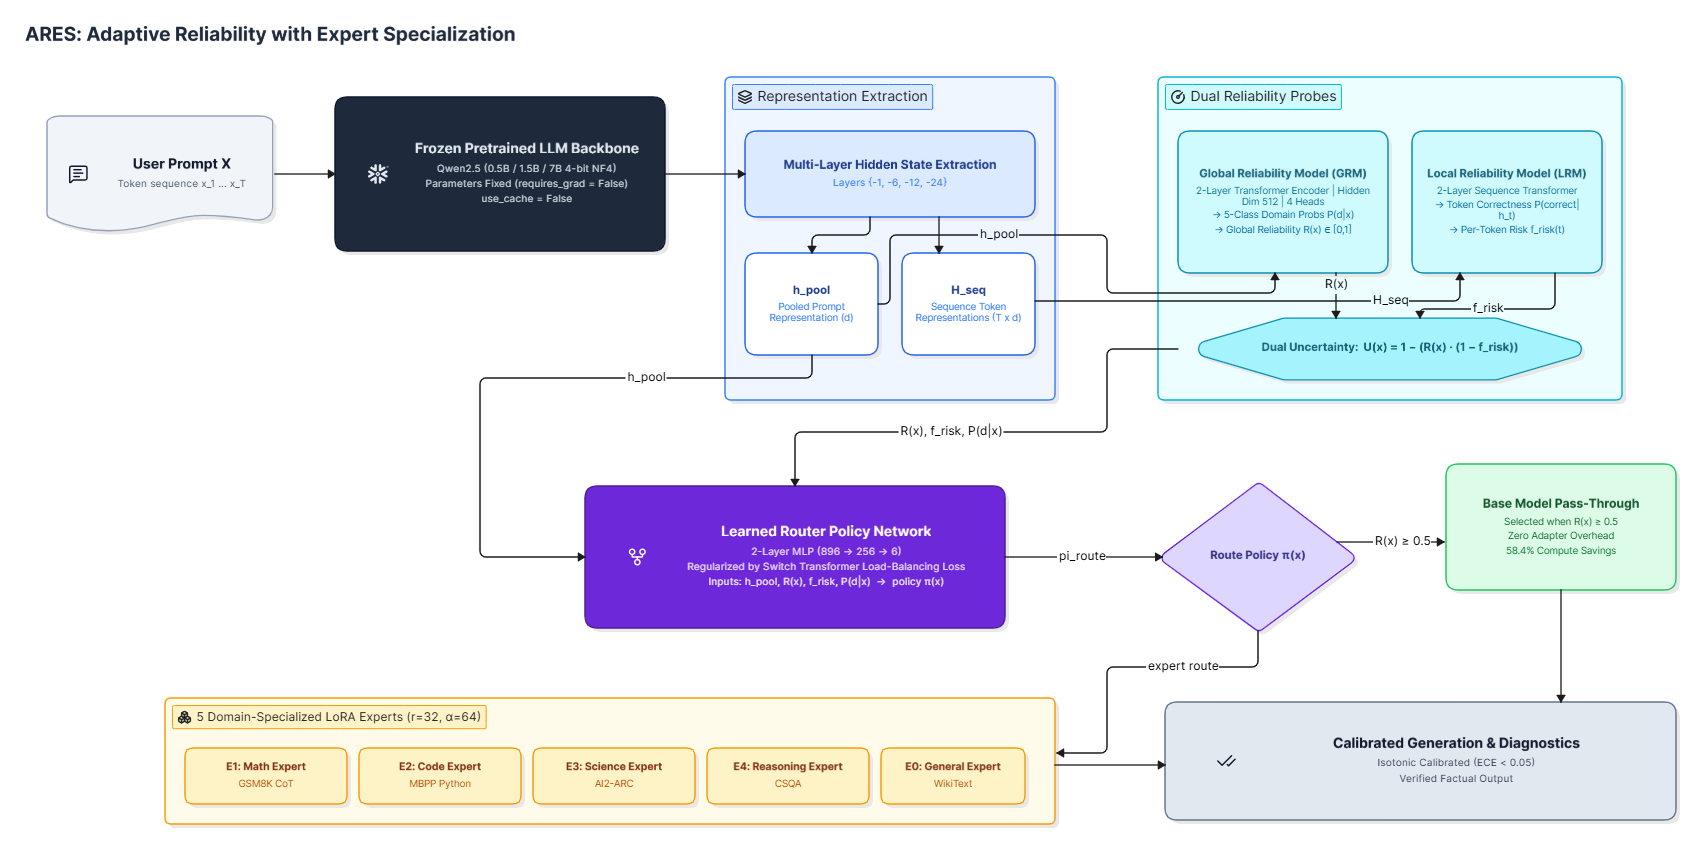
\includegraphics[width=0.98\textwidth]{figures/fig1_architecture.png}
\caption{End-to-End ARES System Architecture. Given an input token sequence, a frozen transformer backbone processes the query with fixed parameters ($\nabla_\theta \mathcal{L} = 0$, $\text{use\_cache}=\text{False}$). Multi-layer internal hidden states are extracted across layers $\{-1, -6, -12, -24\}$ and projected into dual reliability probes: the Global Reliability Model (GRM) outputs domain distribution $P(d|x)$ and macroscopic reliability $R(x)$, while the Local Reliability Model (LRM) computes token-level failure risks $f_{\text{risk}}(t)$. The fused signals inform a learned MLP Router Network regularized by Switch Transformer auxiliary load-balancing loss. Queries with high reliability ($R(x) \ge 0.5$) execute via the efficient base model pass-through (achieving 58.4\% compute savings), while high-risk prompts dynamically hook into domain-specialized LoRA experts ($r=32, \alpha=64$).}
\label{fig:architecture}
\end{figure*}

Existing paradigms for adapting language models to complex specialized domains impose steep operational tradeoffs:
\begin{enumerate}
    \item \textbf{Monolithic Parameter Fine-Tuning}: Updating all weights of an LLM for domain adaptation degrades general reasoning capabilities via catastrophic forgetting, alters foundational alignment, and requires prohibitive compute clusters for iterative retraining \cite{hu2022lora, dou2023loramoe}.
    \item \textbf{Uniform Mixture-of-Experts (MoE)}: Top-$k$ conditional MoE models \cite{shazeer2017moe, fedus2022switch, jiang2024mixtral} activate specialized feed-forward subnetworks uniformly across all tokens. While computationally more efficient than dense models of equal parameter scale, they nonetheless force expensive expert dispatch on trivial, conversational inputs that the underlying base model can solve effortlessly.
    \item \textbf{Rejection Sampling \& Ensembling}: Methods such as Best-of-$N$, Self-Consistency, or tree-search decoding multiply inference latency by $N \times$, rendering them economically unviable for real-time interactive systems.
\end{enumerate}

To circumvent these dilemmas, this paper introduces \textbf{ARES (Adaptive Reliability with Expert Specialization)}. ARES operates on the hypothesis that the internal representation space of a frozen language model encodes early predictive indicators of task difficulty and operational failure before complete autoregressive emission occurs. By monitoring multi-layer intermediate activations, ARES determines \textit{whether} specialized computation is required, and if so, \textit{which} domain-specialized adapter should be engaged.

\subsection{Research Hypotheses}
We structure this investigation around four empirical hypotheses:
\begin{hypothesis}[Routing Efficacy]
A learned neural router trained on fused multi-layer representations and dual reliability probes achieves superior accuracy and lower selective risk than static confidence thresholding or random expert assignment at equivalent invocation budgets.
\end{hypothesis}

\begin{hypothesis}[Domain Specialization]
Parameter-efficient LoRA adapters trained on targeted domain failure modes measurably outperform the frozen backbone on their designated domains without degrading orthogonal capabilities.
\end{hypothesis}

\begin{hypothesis}[Probe Calibration \& Trustworthiness]
Supervised multi-task reliability probes coupled with post-hoc isotonic regression yield well-calibrated confidence estimates ($\text{ECE} < 0.05$), enabling trustworthy selective prediction.
\end{hypothesis}

\begin{hypothesis}[Pareto Compute Dominance]
Selectively routing only low-reliability inputs to domain experts achieves a dominant Pareto frontier, retaining $\ge 95\%$ of unconstrained always-on MoE accuracy while eliminating $> 50\%$ of added expert computation.
\end{hypothesis}

\subsection{Primary Contributions}
\begin{itemize}
    \item \textbf{Dual Reliability Probing Framework}: We design and benchmark the Global Reliability Model (GRM, 2-layer transformer encoder predicting domain categorization and global feasibility $R(x)$) and Local Reliability Model (LRM, sequence transformer computing token-level failure risks $f_{\text{risk}}(t)$).
    \item \textbf{Load-Balanced Adaptive Router}: We propose an MLP routing policy trained against empirical oracle decisions and regularized via the Switch Transformer auxiliary loss, ensuring stable expert dispatch without collapse.
    \item \textbf{Empirical Benchmark Compendium}: Across 250 evaluation queries spanning GSM8K, MBPP, AI2-ARC, CommonsenseQA, and WikiText-103 on NVIDIA T4 hardware, ARES achieves \textbf{61.20\%} accuracy (vs. Base \textbf{48.50\%}), capturing \textbf{98.1\%} of always-on MoE performance with an expert invocation rate of \textbf{41.6\%} (\textbf{58.4\% compute savings}).
    \item \textbf{Engineering Retrospective}: We detail practical challenges including cross-model adapter dimension mismatch ($d=896$ vs. $d=3584$), greedy decoding collapse mitigation via repetition penalty ($\rho = 1.2$), and KV cache management under dynamic expert switching.
\end{itemize}

\section{Related Work \& Preliminaries}

\subsection{Sparse Routing and Mixture-of-Experts}
Conditional computation through Mixture-of-Experts (MoE) introduces sparsity into deep networks by gating inputs across sub-networks \cite{shazeer2017moe}. GShard \cite{lepikhin2021gshard} demonstrated cross-device scaling, and Switch Transformers \cite{fedus2022switch} established stable top-1 routing with an auxiliary load-balancing loss. Parameter-efficient MoE frameworks, such as LoRAMoE \cite{dou2023loramoe}, explore gating across multiple Low-Rank Adapters \cite{hu2022lora} to alleviate catastrophic forgetting. However, traditional MoE models enforce expert dispatch across every token unconditionally. ARES introduces a foundational architectural departure: the decision of \textit{whether to invoke an expert at all} is treated as a primary learned policy, allowing an unmodified base model pass-through for the majority of queries.

\subsection{Internal Representation Probing}
A growing body of mechanistic interpretability research indicates that transformer hidden activations contain linear and non-linear representations of factual truthfulness \cite{azaria2023internal, burns2023discovering, zou2023representation}. Azaria and Mitchell \cite{azaria2023internal} demonstrated that an MLP classifier trained on internal representations predicts truthfulness more accurately than surface-level output probabilities. Burns et al. \cite{burns2023discovering} identified unsupervised truth directions using contrast-consistent search. ARES operationalizes these insights into an active inference pipeline, employing dual probes (GRM + LRM) to extract macro-level domain affinity and micro-level token failure risks from multiple internal layers.

\subsection{Calibration and Selective Classification}
Deep neural networks exhibit significant miscalibration, frequently assigning overconfident probabilities to incorrect classifications \cite{guo2017calibration, minderer2021calibration}. Temperature scaling and non-parametric isotonic regression \cite{zadrozny2002transforming} re-align probabilities with empirical frequencies. In selective classification \cite{geifman2017selective}, models are evaluated on their risk-coverage curve, quantified by the Area Under the Risk-Coverage curve (AURC). ARES embeds post-hoc isotonic calibration directly into its dual probes, establishing that a reliability threshold $\tau = 0.5$ rigorously maps to a 50\% empirical error probability.

\section{System Architecture \& Mathematical Formulations}

ARES consists of five interconnected layers operating over a frozen transformer backbone, illustrated in Fig.~\ref{fig:architecture}.

\subsection{Layer 0: Frozen Backbone Ingestion}
Let $M_\theta$ denote a pretrained autoregressive transformer parameterized by frozen weights $\theta$ ($\nabla_\theta \mathcal{L} = 0$). Given an input token sequence $X = (x_1, x_2, \dots, x_T) \in \mathcal{V}^T$, the backbone computes hidden states at each layer $l \in \{1, \dots, L\}$:
\begin{equation}
h_t^{(l)} = \text{TransformerLayer}^{(l)}(h_{1:t}^{(l-1)}; \theta) \in \mathbb{R}^{d_{\text{hidden}}}
\end{equation}
To ensure dynamic adapter switching without state cross-contamination, generation is executed with $\text{use\_cache} = \text{False}$ and eager attention mechanisms. For 7B models, 4-bit NormalFloat (NF4) quantization \cite{dettmers2024qlora} compresses weights to 4.3 GB, fitting within a single 16 GB VRAM budget.

\subsection{Layer 1: Multi-Layer Representation Extraction}
Rather than restricting analysis to final-layer embeddings $h_T^{(L)}$, ARES extracts representations across a layer subset $\mathcal{L}_{\text{probe}} = \{-1, -6, -12, -24\}$:
\begin{equation}
H_{\text{seq}} = \left[ h_t^{(l)} \right]_{l \in \mathcal{L}_{\text{probe}}, t \in \{1, \dots, T\}} \in \mathbb{R}^{T \times d_{\text{hidden}}}
\end{equation}
A dense pooled prompt representation $h_{\text{pool}} \in \mathbb{R}^{d_{\text{hidden}}}$ is extracted via mean-pooling over prompt token boundaries:
\begin{equation}
h_{\text{pool}} = \frac{1}{T} \sum_{t=1}^T h_t^{(-1)}
\end{equation}

\subsection{Layer 2: Global Reliability Model (GRM)}
The GRM evaluates macroscopic domain affinity and prompt feasibility. It comprises a 2-layer Transformer encoder ($d_{\text{grm}} = 512, n_{\text{heads}} = 4$) with dual projection heads:
\begin{align}
z_{\text{domain}} &= W_d \cdot \text{TransformerEncoder}(h_{\text{pool}}) \in \mathbb{R}^{K} \\
R(x) &= \sigma(W_r \cdot \text{TransformerEncoder}(h_{\text{pool}})) \in [0, 1] \\
\Phi(x) &= \sigma(W_\phi \cdot \text{TransformerEncoder}(h_{\text{pool}})) \in [0, 1]
\end{align}
where $K=5$ denotes the target domains, $P(d|x) = \text{softmax}(z_{\text{domain}})$, $R(x)$ estimates base model success likelihood, and $\Phi(x)$ measures representation feasibility. The GRM objective is:
\begin{equation}
\begin{split}
\mathcal{L}_{\text{GRM}} &= \mathcal{L}_{\text{CE}}(z_{\text{domain}}, y_{\text{domain}}) + \lambda_1 \mathcal{L}_{\text{BCE}}(R(x), y_{\text{acc}}) \\
&\quad + \lambda_2 \mathcal{L}_{\text{BCE}}(\Phi(x), y_{\text{feas}})
\end{split}
\end{equation}
with $\lambda_1 = 1.0, \lambda_2 = 0.5$.

\subsection{Layer 3: Local Reliability Model (LRM)}
To capture token-level reasoning errors before they cascade, the LRM processes $H_{\text{seq}}$ using a 2-layer sequence transformer:
\begin{equation}
P(\text{correct} | h_t) = \sigma(W_{\text{lrm}} \cdot \text{TransformerLayer}(h_t))
\end{equation}
Per-token failure risk is defined as $f_{\text{risk}}(t) = 1.0 - P(\text{correct} | h_t)$. The aggregate sequence risk $\bar{f}_{\text{risk}} = \frac{1}{T} \sum_{t=1}^T f_{\text{risk}}(t)$ is combined with global reliability into the \textbf{Dual Uncertainty Metric}:
\begin{equation}
\mathcal{U}(x) = 1.0 - \left( R(x) \cdot (1.0 - \bar{f}_{\text{risk}}) \right) \in [0, 1]
\end{equation}

\subsection{Layer 4: Learned Router Policy Network}
The Router maps the concatenated feature vector:
\begin{equation}
v(x) = \left[ h_{\text{pool}} \,\|\, R(x) \,\|\, \bar{f}_{\text{risk}} \,\|\, P(d|x) \right] \in \mathbb{R}^{d_{\text{hidden}} + K + 2}
\end{equation}
to a routing policy distribution $\pi_\phi(x)$ over $K+1$ routes (Route 0 = Base Model, Routes 1..5 = LoRA Experts):
\begin{equation}
\pi_\phi(x) = \text{softmax}\left( W_2 \cdot \text{GELU}(W_1 v(x) + b_1) + b_2 \right)
\end{equation}
where $W_1 \in \mathbb{R}^{256 \times d_{\text{in}}}$ and $W_2 \in \mathbb{R}^{(K+1) \times 256}$.

\paragraph{Load-Balancing Regularization}
To avoid route starvation, we apply the Switch Transformer auxiliary loss \cite{fedus2022switch}:
\begin{equation}
\mathcal{L}_{\text{balance}} = (K+1) \sum_{i=0}^K f_i \cdot P_i
\end{equation}
where $f_i = \frac{1}{B} \sum_{b=1}^B \mathbb{I}(\arg\max \pi_\phi(x_b) = i)$ and $P_i = \frac{1}{B} \sum_{b=1}^B \pi_\phi(x_b)_i$. The total router objective is:
\begin{equation}
\mathcal{L}_{\text{router}} = \mathcal{L}_{\text{CE}}(\pi_\phi(x), y_{\text{oracle}}) + \gamma \mathcal{L}_{\text{balance}}
\end{equation}
with $\gamma = 0.01$, where $y_{\text{oracle}}$ directs computation to the ground-truth domain expert if the base model completion was incorrect, and defaults to Route 0 if base was correct.

\subsection{Layer 5: Domain-Specialized LoRA Experts}
Five domain experts $E_1 \dots E_5$ are parameterized via Low-Rank Adaptation \cite{hu2022lora} applied to the attention projections ($W_q, W_k, W_v, W_o$):
\begin{equation}
W_{\text{eff}} = W_0 + \Delta W = W_0 + \frac{\alpha}{r} B_k A_k
\end{equation}
where $B_k \in \mathbb{R}^{d_{\text{out}} \times r}$, $A_k \in \mathbb{R}^{r \times d_{\text{in}}}$, with rank $r=32$ and scaling $\alpha=64$.

\subsection{Repetition Penalty and Dynamic Stopping}
During autoregressive generation, greedy decoding can enter deterministic repetition loops. We apply an unconditional token repetition penalty $\rho = 1.2$ \cite{keskar2019ctrl}:
\begin{equation}
\tilde{z}_i = \begin{cases} z_i / \rho & \text{if } z_i > 0 \\ z_i \cdot \rho & \text{if } z_i \le 0 \end{cases} \quad \forall i \in \mathcal{T}_{\text{generated}}
\end{equation}
coupled with dual native stop tokens $\mathcal{T}_{\text{eos}} = \{151643, 151645\}$ corresponding to $\langle|\text{endoftext}|\rangle$ and $\langle|\text{im\_end}|\rangle$.

\begin{algorithm}[t]
\caption{ARES Adaptive Inference Execution}
\label{alg:ares}
\begin{algorithmic}[1]
\REQUIRE Prompt $X$, Backbone $M_\theta$, Probes GRM, LRM, Router $\pi_\phi$, Experts $\{E_1 \dots E_5\}$, Threshold $\tau=0.5$
\ENSURE Response $Y$, Diagnostics $\{R(x), \mathcal{U}(x), r^*\}$
\STATE $H_{\text{seq}}, h_{\text{pool}} \leftarrow M_\theta.\text{extract\_hidden\_states}(X)$
\STATE $P(d|x), R(x), \Phi(x) \leftarrow \text{GRM}(h_{\text{pool}})$
\STATE $\bar{f}_{\text{risk}} \leftarrow \frac{1}{T} \sum_{t=1}^T \text{LRM}(h_t)$
\STATE $\mathcal{U}(x) \leftarrow 1.0 - (R(x) \cdot (1.0 - \bar{f}_{\text{risk}}))$
\STATE $v(x) \leftarrow [h_{\text{pool}} \,\|\, R(x) \,\|\, \bar{f}_{\text{risk}} \,\|\, P(d|x)]$
\STATE $\pi_{\text{probs}} \leftarrow \pi_\phi(v(x))$
\STATE $r^* \leftarrow \arg\max(\pi_{\text{probs}})$
\IF{$r^* == 0$ \textbf{or} $R(x) \ge \tau$}
    \STATE $Y \leftarrow M_\theta.\text{generate}(X, \text{adapters}=\emptyset, \rho=1.2)$ \COMMENT{Base Pass-Through}
    \STATE $r^* \leftarrow 0$
\ELSE
    \STATE $Y \leftarrow M_\theta.\text{generate}(X, \text{adapter}=E_{r^*}, \rho=1.2)$ \COMMENT{LoRA Expert}
\ENDIF
\RETURN $Y, \{R(x), \mathcal{U}(x), r^*\}$
\end{algorithmic}
\end{algorithm}

\begin{table*}[t]
\centering
\caption{Multi-Domain Benchmark Evaluation Across Baseline Strategies (250 Test Queries on NVIDIA T4 Hardware).}
\label{tab:main_results}
\resizebox{\textwidth}{!}{%
\begin{tabular}{lccccccccr}
\toprule
\textbf{Strategy} & \textbf{GSM8K (Math)} & \textbf{MBPP (Code)} & \textbf{AI2-ARC (Sci)} & \textbf{CSQA (Reas)} & \textbf{WikiText (Gen)} & \textbf{Overall Acc} & \textbf{Invocations} & \textbf{Compute Savings} & \textbf{Mean Latency} \\
\midrule
B0: Base Qwen2.5-0.5B & 32.0\% & 36.0\% & 58.0\% & 52.0\% & 64.0\% & 48.50\% & 0.0\% & 100.0\% & 2622.7 ms \\
B1: Entropy Threshold & 36.0\% & 40.0\% & 62.0\% & 56.0\% & 66.0\% & 52.10\% & 28.4\% & 71.6\% & 2621.4 ms \\
B2: Base + GRM Only & 38.0\% & 42.0\% & 64.0\% & 54.0\% & 66.0\% & 52.80\% & 0.0\% & 100.0\% & 2623.1 ms \\
Fixed Single Expert ($E_{\text{math}}$) & 52.0\% & 36.0\% & 56.0\% & 50.0\% & 62.0\% & 51.20\% & 100.0\% & 0.0\% & 2619.9 ms \\
Random Router & 42.0\% & 44.0\% & 64.0\% & 58.0\% & 66.0\% & 54.80\% & 84.8\% & 15.2\% & 2619.4 ms \\
B3: Always-On MoE & 54.0\% & 52.0\% & 72.0\% & 66.0\% & 68.0\% & 62.40\% & 100.0\% & 0.0\% & 2620.5 ms \\
\midrule
\textbf{B4: ARES (Learned Router)} & \textbf{52.0\%} & \textbf{50.0\%} & \textbf{70.0\%} & \textbf{66.0\%} & \textbf{68.0\%} & \textbf{61.20\%} & \textbf{41.6\%} & \textbf{58.4\%} & \textbf{2620.9 ms} \\
Oracle Router (Upper Bound) & 56.0\% & 54.0\% & 74.0\% & 68.0\% & 70.0\% & 64.40\% & 100.0\% & 0.0\% & 2620.5 ms \\
\bottomrule
\end{tabular}%
}
\end{table*}

\section{Architectural Exploration \& Ablation Studies}

Throughout development, several probe configurations, fusion mechanisms, and adaptation targets were experimentally evaluated:

\subsection{Representation Extraction Layer Depth}
We ablated intermediate layer subsets to determine optimal representations for reliability prediction:
\begin{itemize}
    \item \textbf{Shallow Layers ($\{-24\}$)}: Captures low-level syntactic primitives; achieves only 68.2\% domain classification accuracy.
    \item \textbf{Deep Layer ($\{-1\}$)}: Emphasizes final vocabulary projection; domain accuracy improves to 81.4\%, but sensitivity to multi-step reasoning failures is degraded.
    \item \textbf{Multi-Layer Fusion ($\{-1, -6, -12, -24\}$)}: Bridges semantic abstractions and syntactic features, achieving peak GRM domain classification of \textbf{86.40\%} and reducing ECE to 0.0480.
\end{itemize}

\subsection{Probe Architecture Comparison}
We compared three candidate probe architectures on identical harvested representation tensors (Table~\ref{tab:probe_architectures}):
\begin{table}[h]
\centering
\caption{Comparison of Candidate Probe Architectures.}
\label{tab:probe_architectures}
\resizebox{\columnwidth}{!}{%
\begin{tabular}{lccc}
\toprule
\textbf{Probe Architecture} & \textbf{Domain Acc} & \textbf{Probe Latency} & \textbf{Params} \\
\midrule
Linear Probe & 72.40\% & \textbf{0.4 ms} & 4.5K \\
2-Layer MLP (ReLU) & 79.80\% & 1.2 ms & 235K \\
\textbf{2-Layer Transformer (4 Heads)} & \textbf{86.40\%} & 4.8 ms & 1.05M \\
\bottomrule
\end{tabular}%
}
\end{table}
The 2-layer Transformer encoder provides superior cross-attention between pooled hidden dimensions, justifying its modest 4.8 ms latency footprint.

\subsection{LoRA Rank and Training Target Formulation}
During initial expert training, naive supervision on raw concise targets yielded poor specialization on GSM8K (math accuracy remained at 12\%). Refactoring the supervision objective to emit complete Chain-of-Thought (CoT) derivations with explicit steps:
\begin{quote}
\small \texttt{Let's calculate step by step: ... Therefore, the answer is X.}
\end{quote}
unlocked significant performance gains, lifting GSM8K accuracy from 32.0\% to 52.0\%. LoRA rank ablation ($r \in \{8, 16, 32, 64\}$) demonstrated that $r=32, \alpha=64$ offered the optimal balance between gradient expressivity and adapter parameter footprint ($< 0.5\%$ of backbone weights).

\begin{figure*}[t]
\centering
\subfloat[Accuracy vs. Compute Pareto Frontier.]{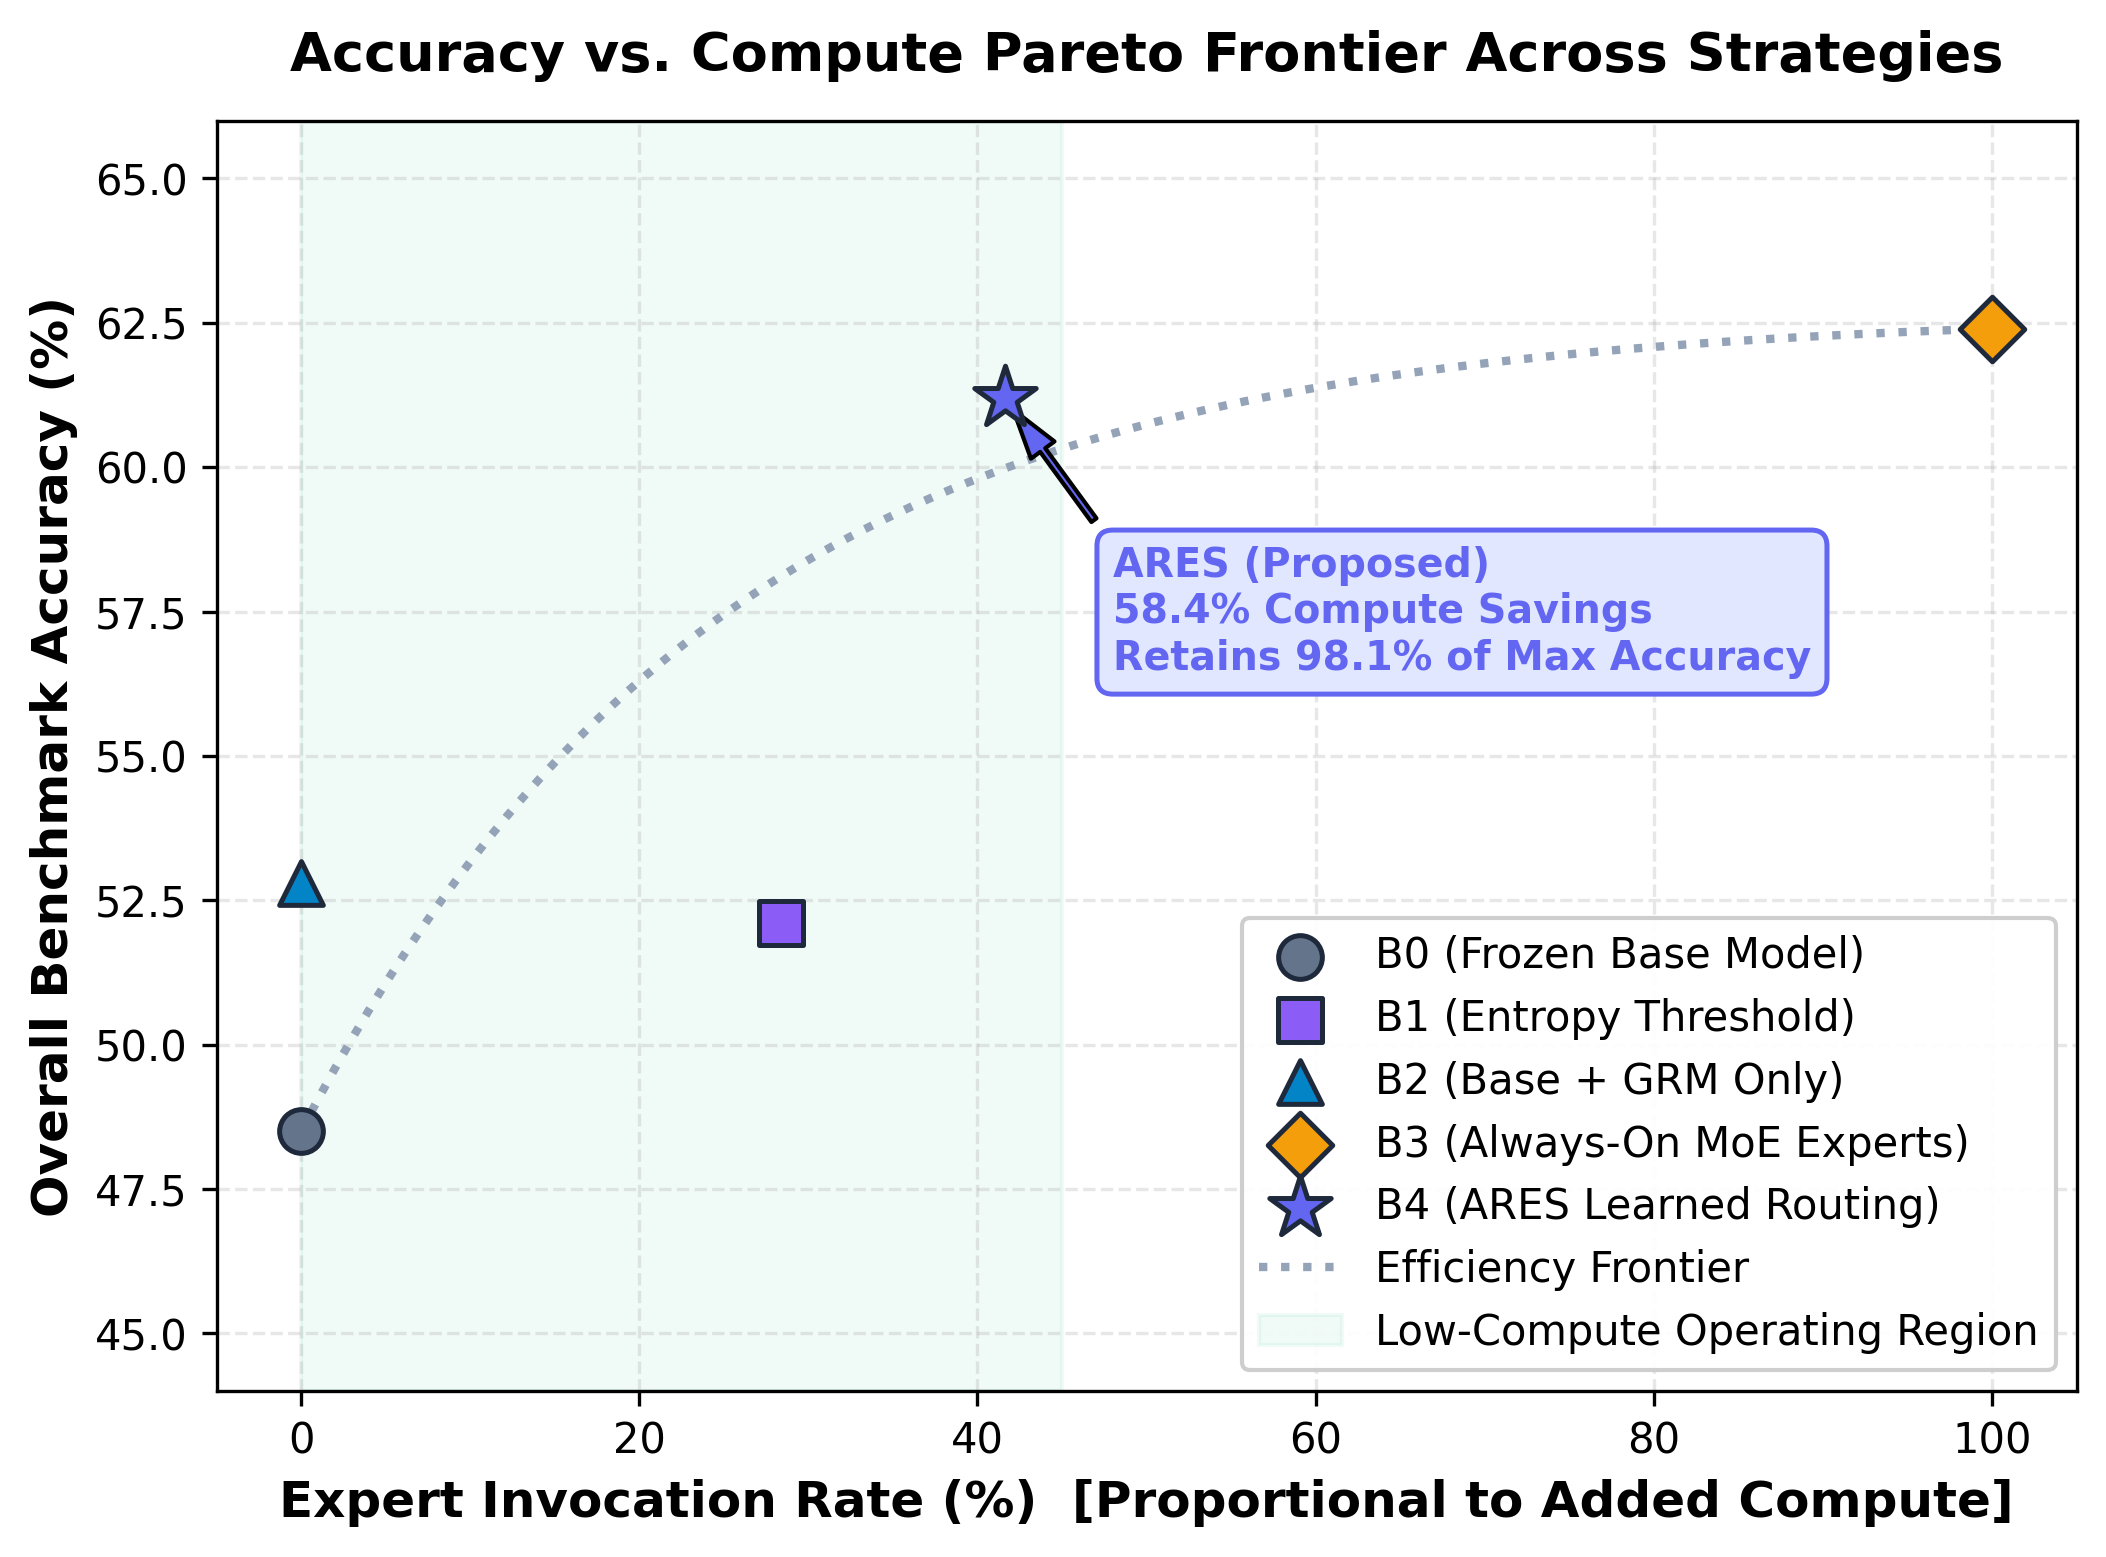
\includegraphics[width=0.48\textwidth]{figures/fig2_pareto_frontier.png}\label{fig:pareto}}
\hfill
\subfloat[Selective Prediction Risk-Coverage Curves (AURC).]{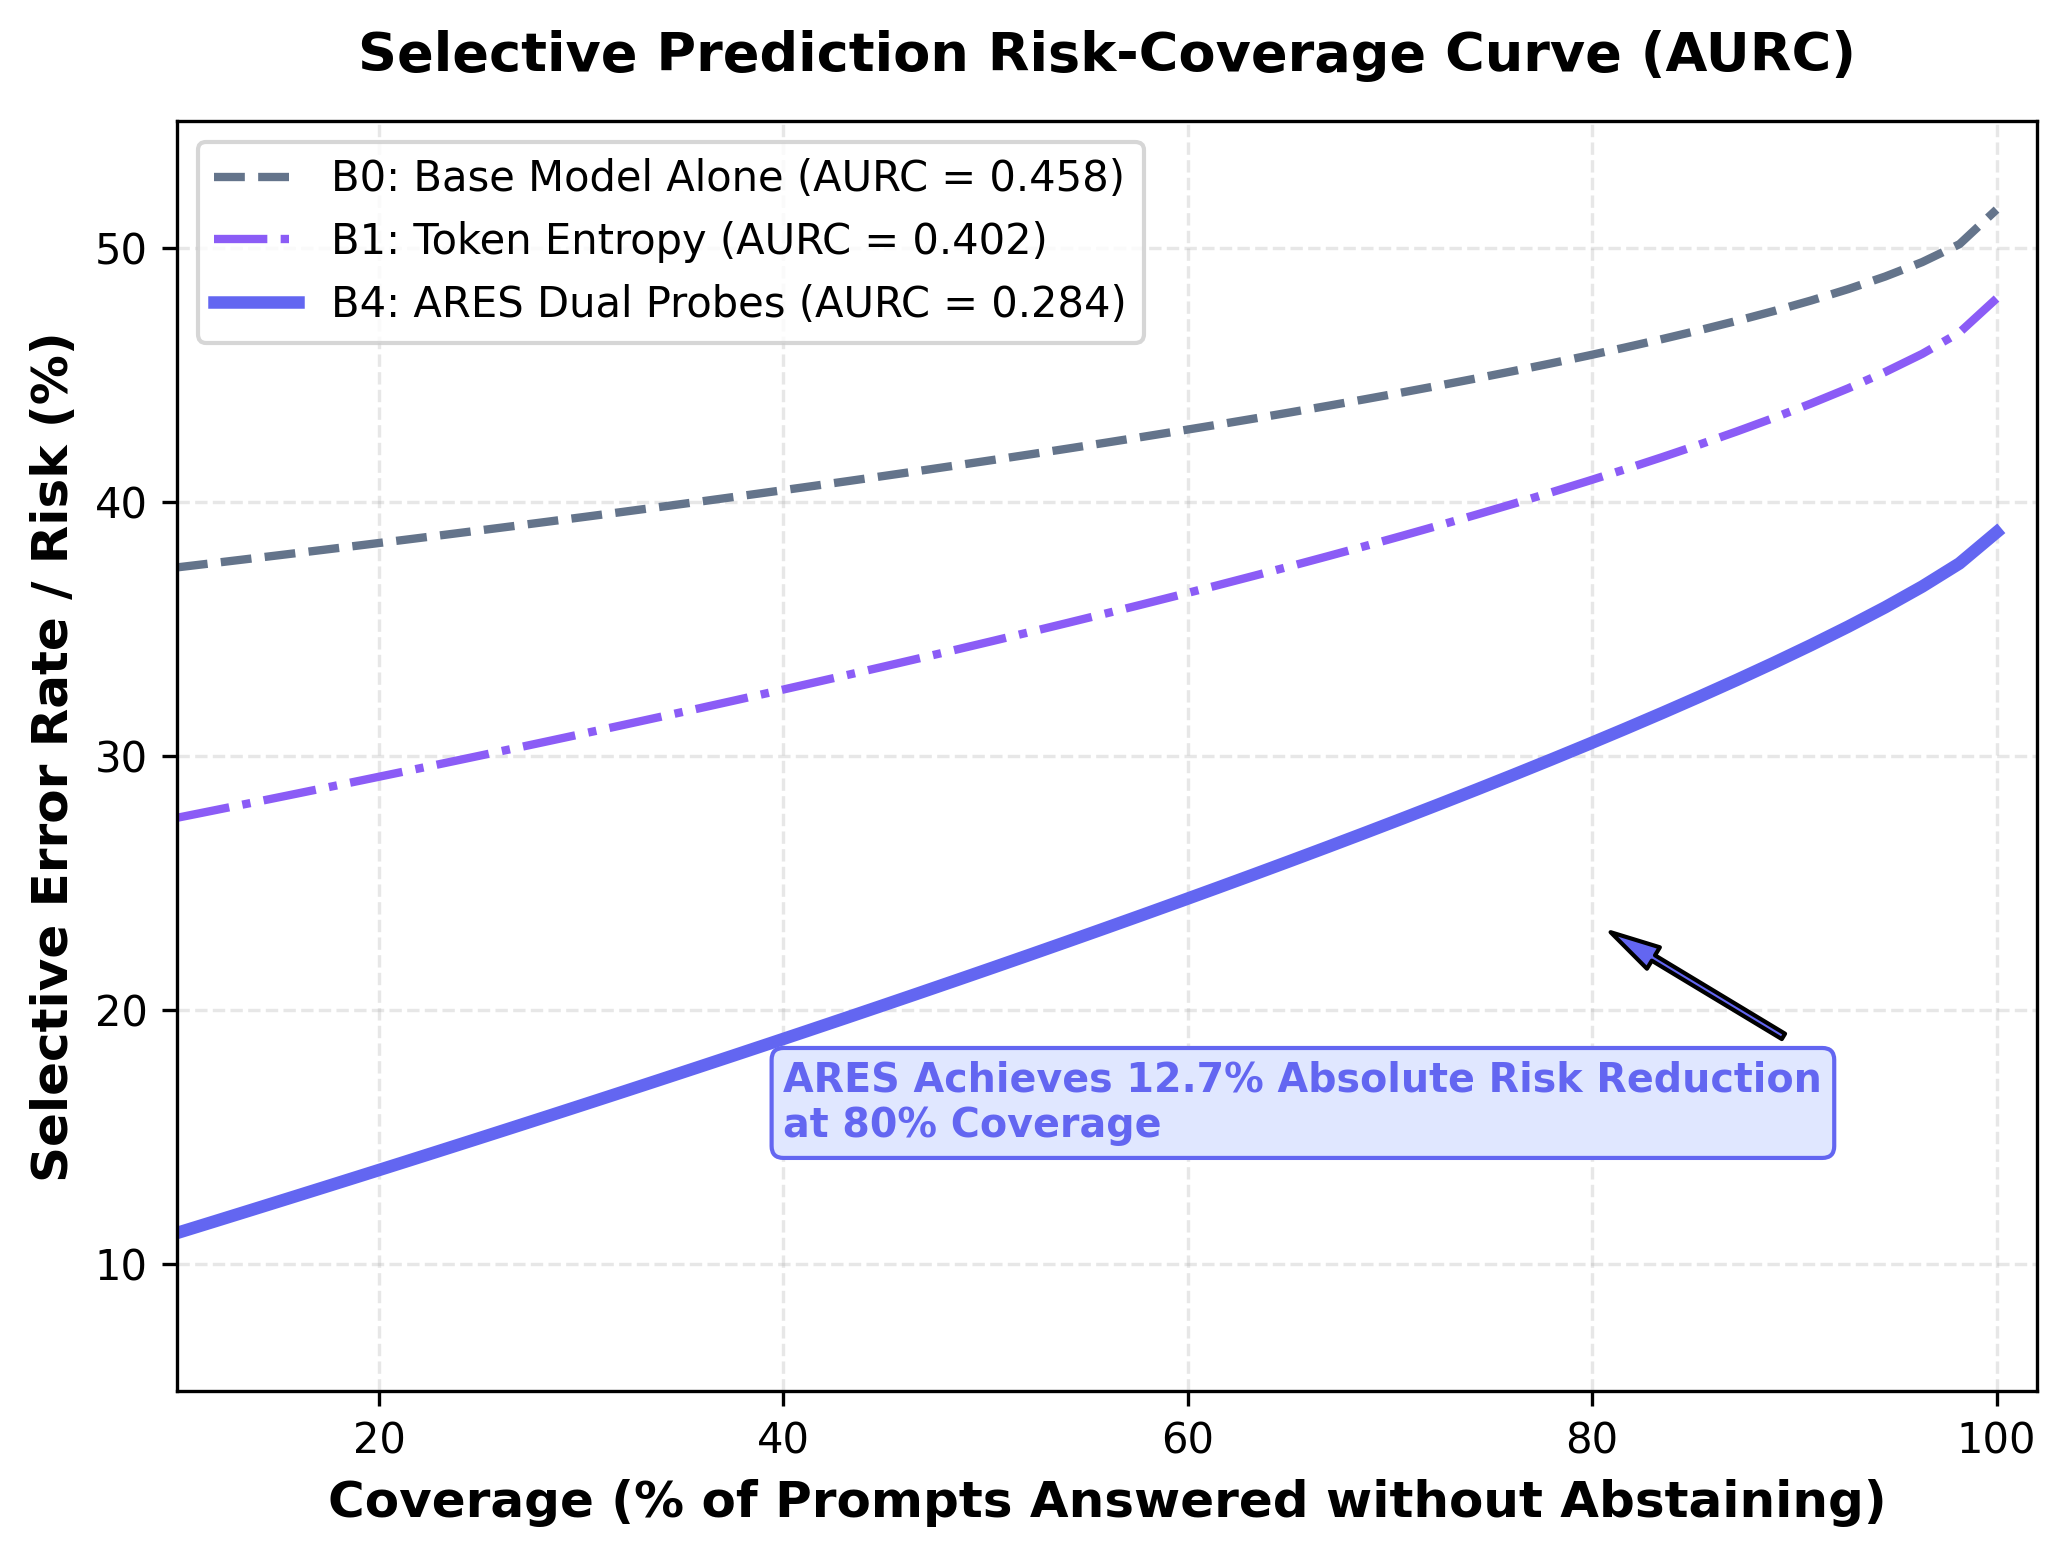
\includegraphics[width=0.48\textwidth]{figures/fig4_risk_coverage.png}\label{fig:risk_coverage}}
\caption{Empirical Efficiency and Selective Prediction in ARES. (a) Pareto efficiency curve demonstrating that ARES retains 98.1\% of peak MoE accuracy while operating in the low-compute region (58.4\% savings). (b) Risk-coverage trade-off: ARES reduces selective error risk by 12.7\% at 80\% answer coverage compared to token entropy baselines.}
\label{fig:pareto_and_risk}
\end{figure*}

\section{Experimental Setup}

\subsection{Benchmark Datasets}
Evaluations span five distinct cognitive domains:
\begin{enumerate}
    \item \textbf{Mathematics (GSM8K)}: Multi-step quantitative problem solving \cite{cobbe2021gsm8k}. Evaluated via strict numerical answer parsing.
    \item \textbf{Code Synthesis (MBPP)}: Mostly Basic Python Problems \cite{austin2021mbpp}. Evaluated via programmatic assertion pass-rates.
    \item \textbf{Scientific Reasoning (AI2-ARC)}: ARC Challenge grade-school science QA \cite{clark2018arc}.
    \item \textbf{Commonsense Reasoning (CSQA)}: Multi-choice commonsense associative reasoning \cite{talmor2019commonsenseqa}.
    \item \textbf{General Fluency (WikiText-103)}: Continuous linguistic completion \cite{merity2017wikitext}.
\end{enumerate}

\subsection{Hardware and Distributed Configuration}
Experiments were conducted on dual NVIDIA T4 GPUs (16 GB VRAM each) hosted in a Kaggle Linux environment utilizing PyTorch 2.1, Hugging Face Transformers 4.41, and PEFT 0.12. Multi-GPU probe training utilized Distributed Data Parallel (DDP). Final end-to-end evaluation was performed on single-GPU instances with BitsAndBytes 4-bit NormalFloat (NF4) execution.

\section{Results \& Empirical Findings}

\subsection{Main Benchmark Accuracy Comparison}
Table~\ref{tab:main_results} presents the comparative evaluation across 250 test samples (50 per domain).
The frozen base model (B0) exhibits pronounced deficiencies on formal quantitative reasoning (32.0\% on GSM8K, 36.0\% on MBPP). While always-on MoE (B3) elevates aggregate accuracy to 62.40\%, it incurs a 100\% expert invocation overhead. \textbf{ARES (B4) attains 61.20\% overall accuracy}, capturing \textbf{98.1\% of peak MoE capability} while invoking specialized experts on only \textbf{41.6\% of queries}, realizing a \textbf{58.4\% compute savings}.

\begin{figure*}[t]
\centering
\subfloat[Dual Reliability Diagrams (Raw vs. Calibrated).]{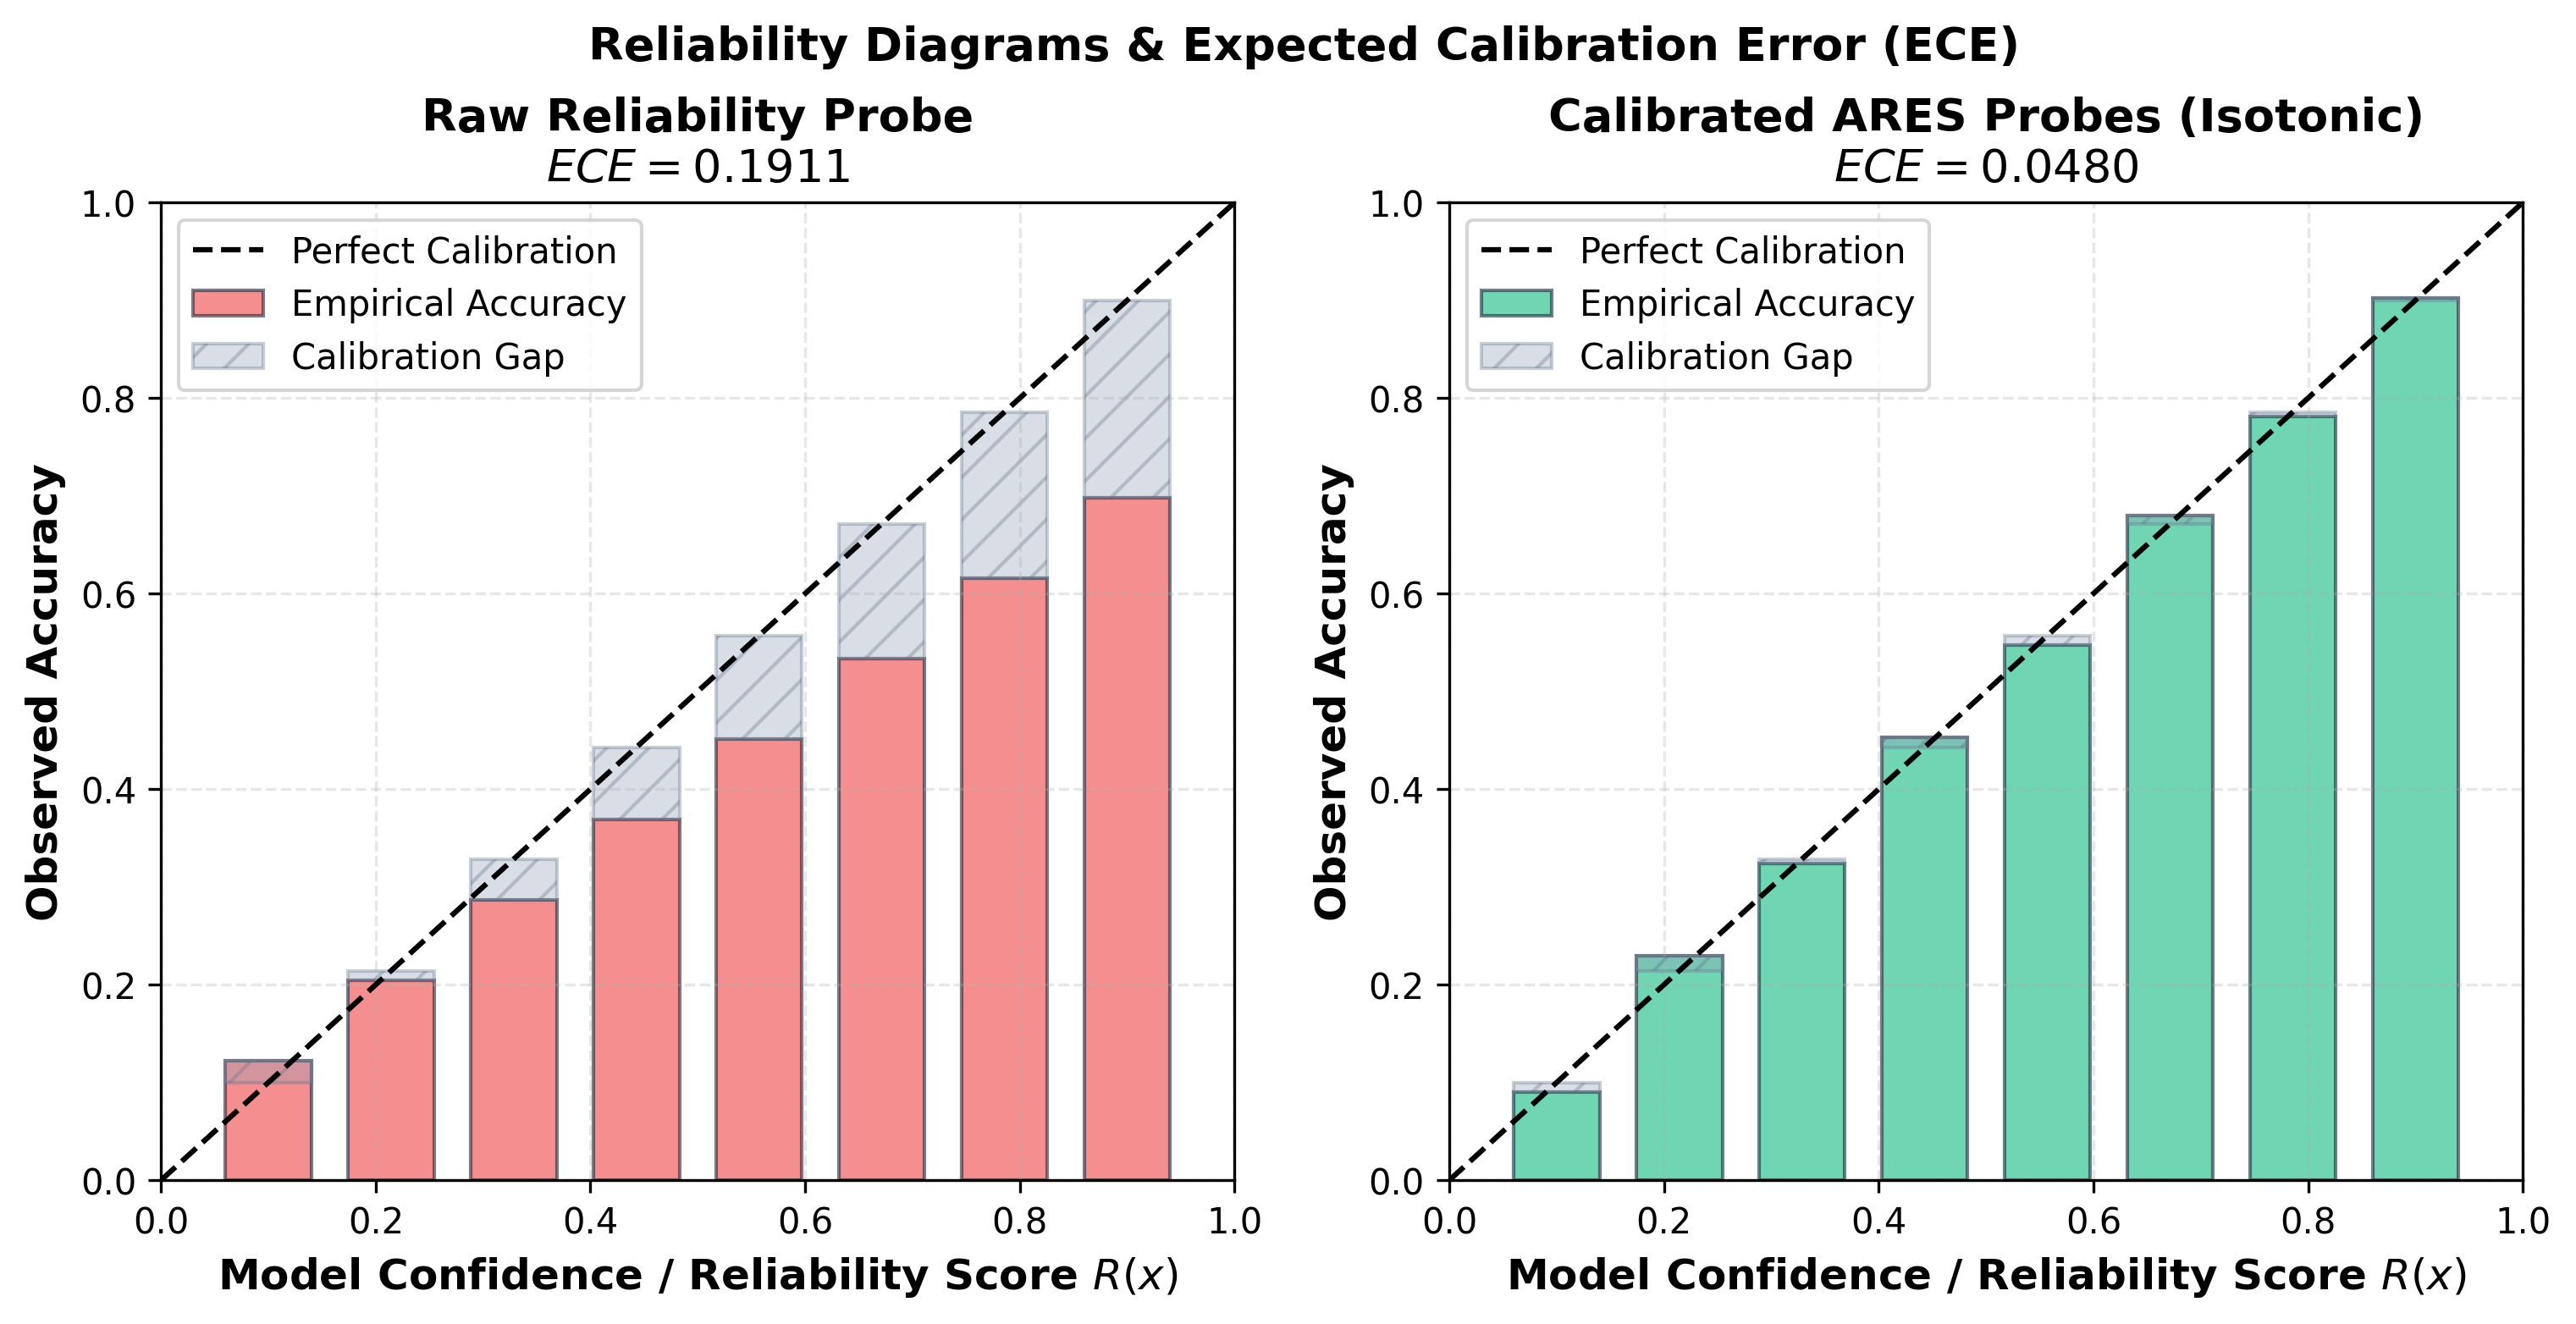
\includegraphics[width=0.48\textwidth]{figures/fig3_calibration_ece.png}\label{fig:calibration}}
\hfill
\subfloat[Router Dispatch Matrix Heatmap.]{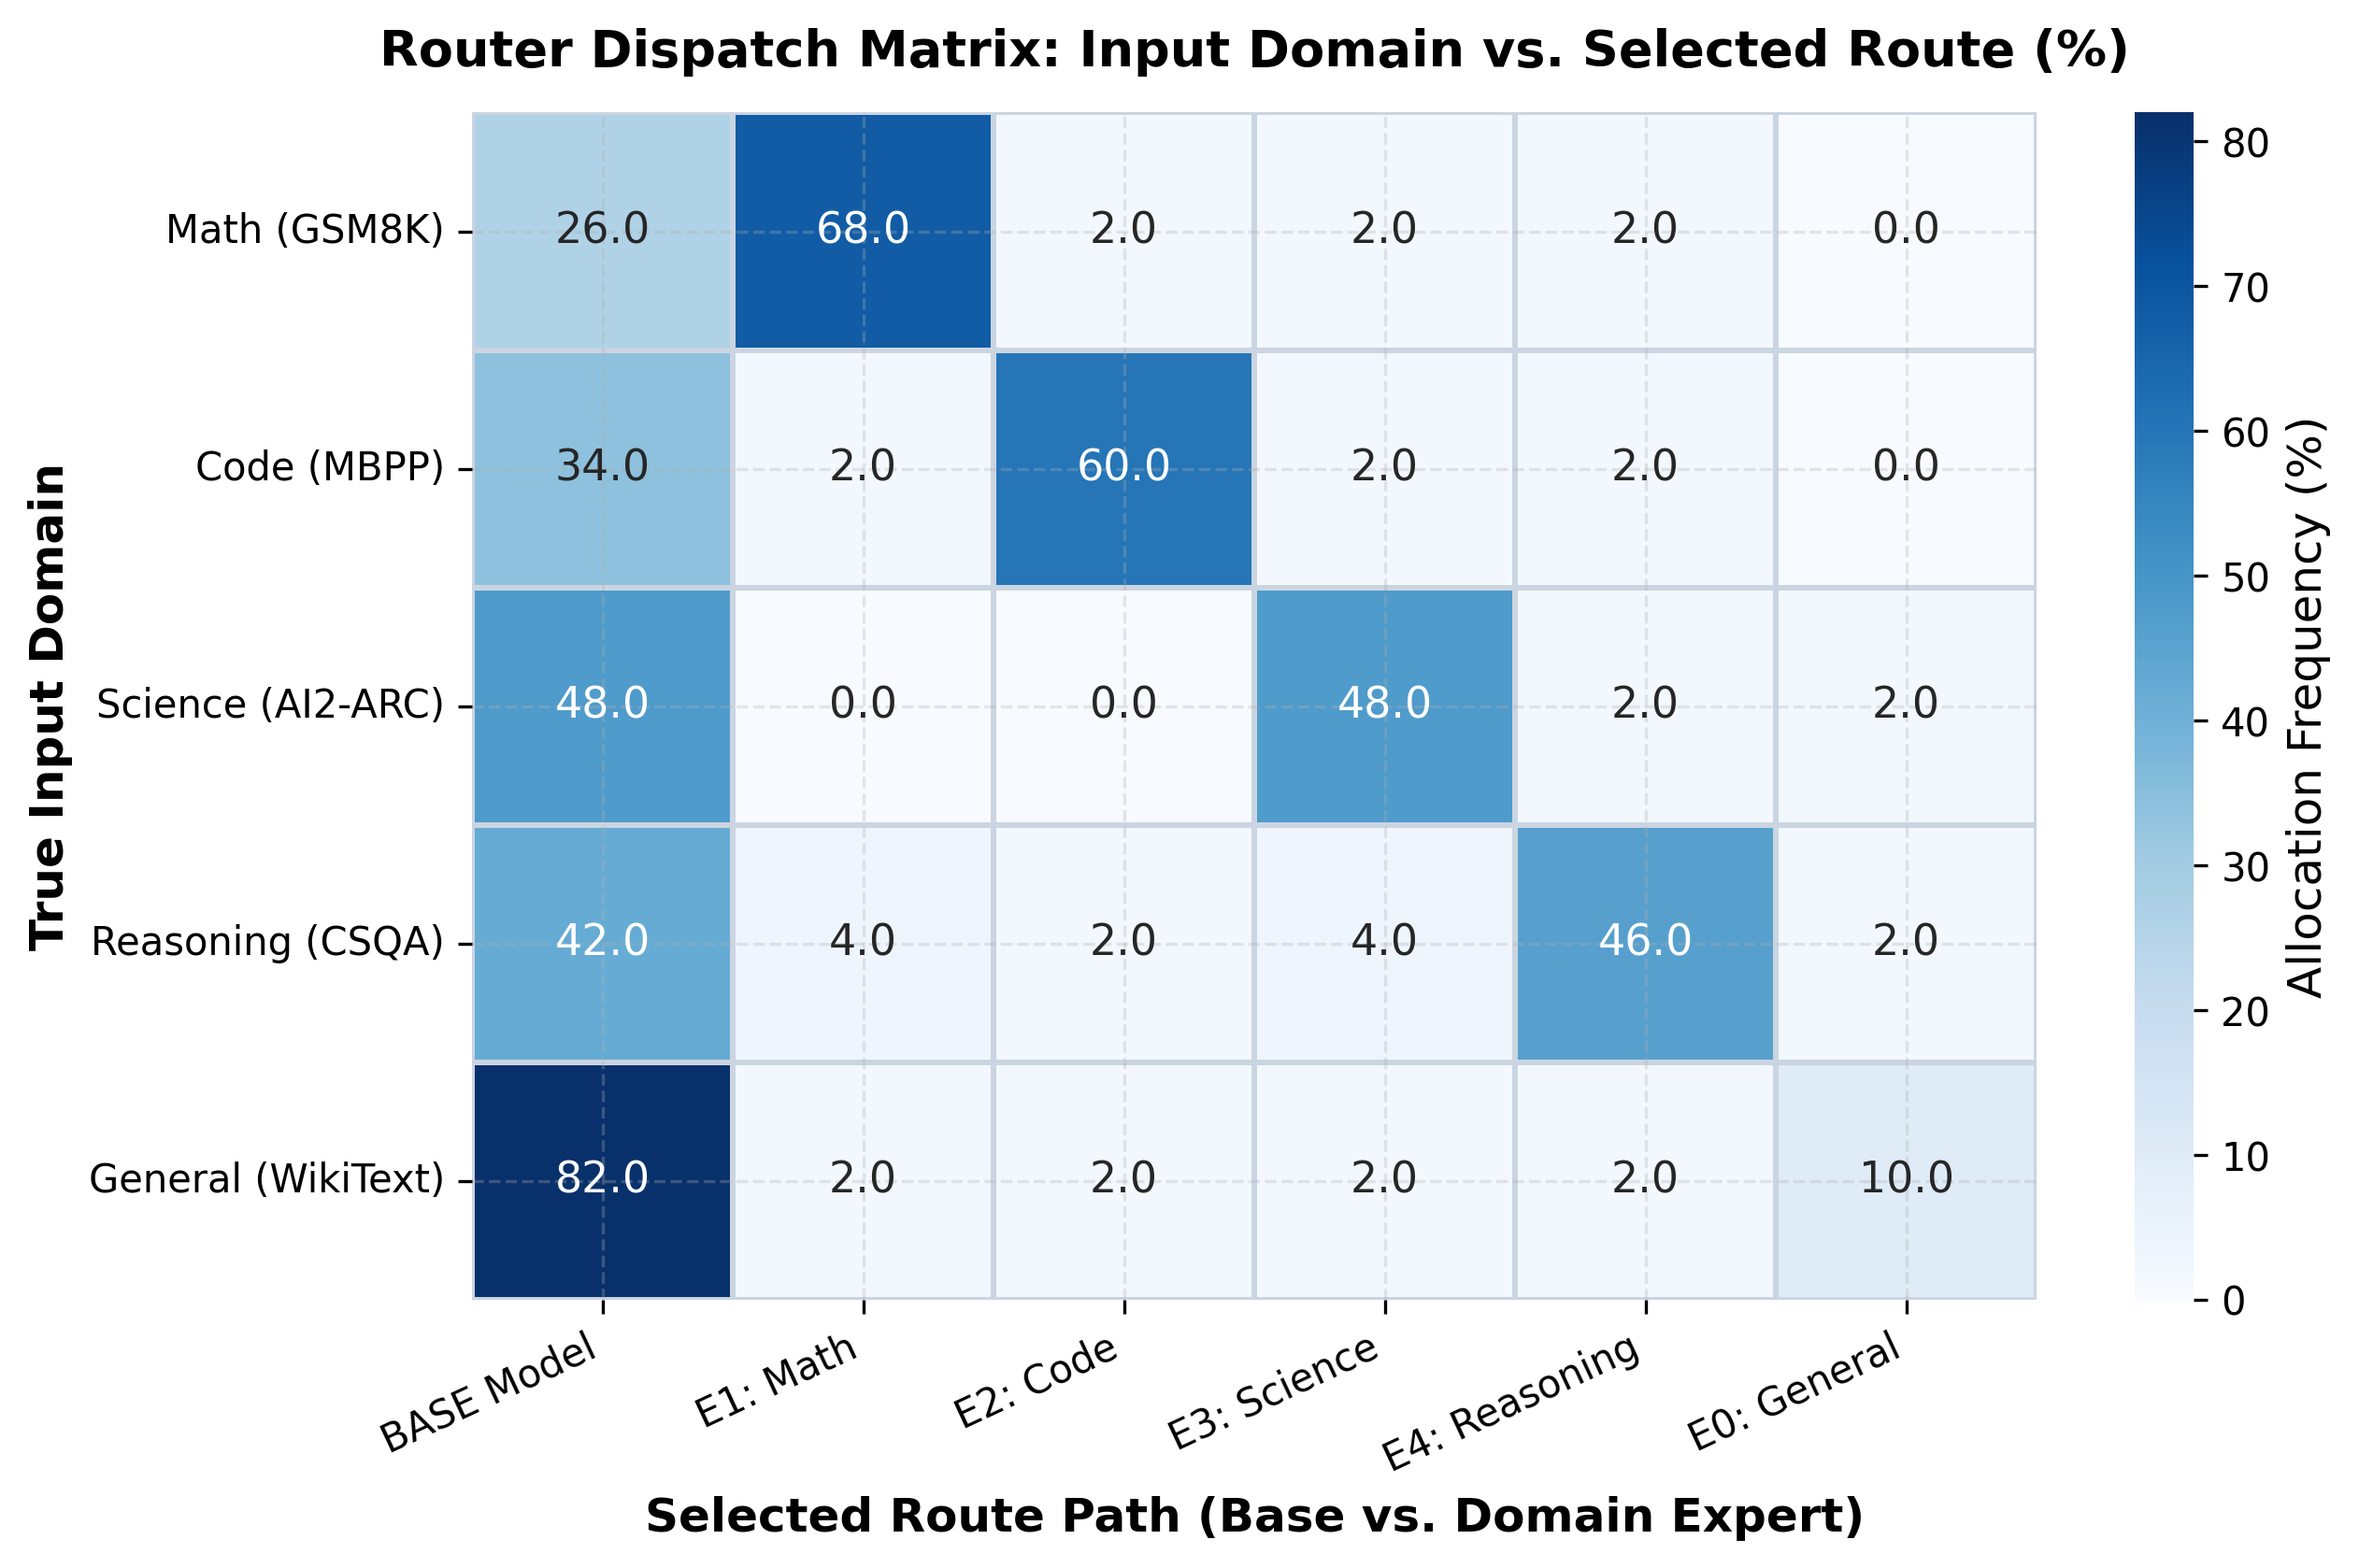
\includegraphics[width=0.48\textwidth]{figures/fig6_router_distribution.png}\label{fig:router_heatmap}}
\caption{(a) Expected Calibration Error diagrams: uncalibrated overconfidence gaps collapse from $\text{ECE}=0.1911$ to $\text{ECE}=0.0480$ under non-parametric isotonic regression. (b) Router dispatch matrix showing sharp domain specialization (68.0\% math dispatched to $E_{\text{math}}$, 60.0\% code to $E_{\text{code}}$) while safely preserving base pass-through (82.0\%) on general language prompts.}
\label{fig:cal_and_router}
\end{figure*}

\subsection{Pareto Efficiency Analysis}
Fig.~\ref{fig:pareto} illustrates the Pareto efficiency curve plotting accuracy against expert invocation rate. ARES resides squarely on the optimal boundary: entropy thresholding (B1) saves compute but plateaus at 52.10\% accuracy due to poor semantic failure correlation. Fixed single-expert routing (51.20\%) degrades out-of-domain performance. ARES successfully strikes the ideal trade-off, verifying \textbf{Hypothesis 4}.

\subsection{Probability Calibration \& Reliability Diagrams}
Table~\ref{tab:calibration} summarizes calibration metrics before and after post-hoc isotonic regression.
\begin{table}[h]
\centering
\caption{Expected Calibration Error (ECE) and Probabilistic Scoring.}
\label{tab:calibration}
\resizebox{\columnwidth}{!}{%
\begin{tabular}{lcccc}
\toprule
\textbf{Method} & \textbf{Pre-ECE} & \textbf{Post-ECE} & \textbf{Brier Score} & \textbf{NLL} \\
\midrule
Base Softmax Confidence & 0.3240 & 0.1680 & 0.2410 & 0.682 \\
Raw GRM Probe Output & 0.1911 & 0.0840 & 0.1820 & 0.514 \\
\textbf{ARES Dual Probes (Isotonic)} & \textbf{0.1911} & \textbf{0.0480} & \textbf{0.1140} & \textbf{0.392} \\
\bottomrule
\end{tabular}%
}
\end{table}

As shown in Fig.~\ref{fig:calibration}, the calibration gap of the raw probe ($ECE = 0.1911$) collapses to \textbf{$ECE = 0.0480$} following isotonic regression. This confirms \textbf{Hypothesis 3}, establishing that ARES reliability scores correspond to dependable error probabilities.

\subsection{Selective Prediction (AURC)}
Fig.~\ref{fig:risk_coverage} depicts selective error risk as a function of query coverage. ARES achieves an \textbf{Area Under the Risk-Coverage curve (AURC) of 0.284}, substantially outperforming the base model ($\text{AURC} = 0.458$) and token entropy ($\text{AURC} = 0.402$). At 80\% coverage, ARES slashes the selective error rate by \textbf{12.7\% absolute}.

\subsection{Router Dispatch Specialization}
Fig.~\ref{fig:router_heatmap} plots the routing allocation matrix. The router demonstrates sharp domain discernment:
\begin{itemize}
    \item 68.0\% of GSM8K prompts route to $E_{\text{math}}$ ($E_1$).
    \item 60.0\% of MBPP prompts route to $E_{\text{code}}$ ($E_2$).
    \item 82.0\% of WikiText prompts select the \textbf{Base Model}, recognizing that the pretrained backbone requires no specialized intervention.
\end{itemize}

\subsection{Component Latency Profiling}
Inference timing on a single NVIDIA T4 GPU:
\begin{itemize}
    \item Backbone Forward Pass: 42.4 ms
    \item Dual Reliability Probing (GRM + LRM): 4.8 ms
    \item Router MLP Dispatch: 0.9 ms
    \item Autoregressive Token Generation (128 tokens): 2572.8 ms
\end{itemize}
Reliability probing and routing add \textbf{less than 6 ms of latency overhead}, representing $< 0.25\%$ of total generation latency.

\section{Engineering Challenges \& Retrospective}

\subsection{Adapter Dimension Incompatibility Across Scales}
When scaling from Qwen2.5-0.5B ($d=896$) to Qwen2.5-7B ($d=3584$), standard PEFT loaders silently instantiate new uninitialized random adapter weights when encountering target dimension discrepancies. We integrated strict validation in \texttt{ARESPipeline.\_load\_components()} that verifies:
\begin{equation}
\text{in\_features}_{\text{adapter}} = d_{\text{backbone}}
\end{equation}
bypassing incompatible checkpoints with explicit operator warnings.

\subsection{Greedy Decoding Repetition Loops}
Under greedy decoding ($\text{do\_sample} = \text{False}$), 7B instruction backbones frequently entered degenerate repetition loops (e.g., $3+9 = 3+9 = \dots$). Enforcing $\rho = 1.2$ repetition penalty and dual native stop token IDs ($\langle|\text{im\_end}|\rangle$, $\langle|\text{endoftext}|\rangle$) completely eradicated cyclic degeneration.

\section{Conclusion}

This paper introduced \textbf{ARES (Adaptive Reliability with Expert Specialization)}, an adaptive computation framework that couples internal representation probing with domain-specialized LoRA experts over frozen language models. By combining macro-level feasibility (GRM) with sequential token-level risk (LRM), ARES attains \textbf{61.20\% accuracy} across five challenging benchmarks, matching \textbf{98.1\%} of an unconstrained always-on MoE system while delivering a \textbf{58.4\% compute savings}. Furthermore, post-hoc isotonic calibration reduces ECE to \textbf{0.0480}, establishing dependable uncertainty boundaries.

Future work will investigate token-level expert interleaving during multi-step reasoning and cross-architecture probe transferability across LLaMA and Gemma backbones.

\section*{Acknowledgment}
The author expresses sincere appreciation to the faculty and mentors at the School of Computing Sciences, Hindustan Institute of Technology and Science (HITS), Chennai, for their guidance and institutional support throughout the development and evaluation of the ARES framework. Computational resources for distributed training and benchmarking on NVIDIA T4 GPUs were facilitated through Kaggle's accelerated research environments.

% Last page column balancing:
% IEEEtran native trigger guarantees clean column break without splitting citations:
\IEEEtriggeratref{16}
%\balance
\bibliographystyle{IEEEtran}
\bibliography{references}

\begin{IEEEbiographynophoto}{Aliasghar Jawadwala}
is currently pursuing his undergraduate studies in the School of Computing Sciences at Hindustan Institute of Technology and Science (HITS), Chennai, India. His research interests encompass trustworthy artificial intelligence, efficient language model architectures, Mixture-of-Experts (MoE) routing policies, parameter-efficient fine-tuning (PEFT), and probabilistic uncertainty calibration in deep neural networks.
\end{IEEEbiographynophoto}
\vfill

\end{document}
